\section{Introduction}%
\pagenumbering{arabic}
\setcounter{page}{1}

\newcounter{x}

\vspace{1cm}

\begin{figure}[h]
  \label{fig:paradise}
  \centering
  \fcolorbox{black}{white}{
    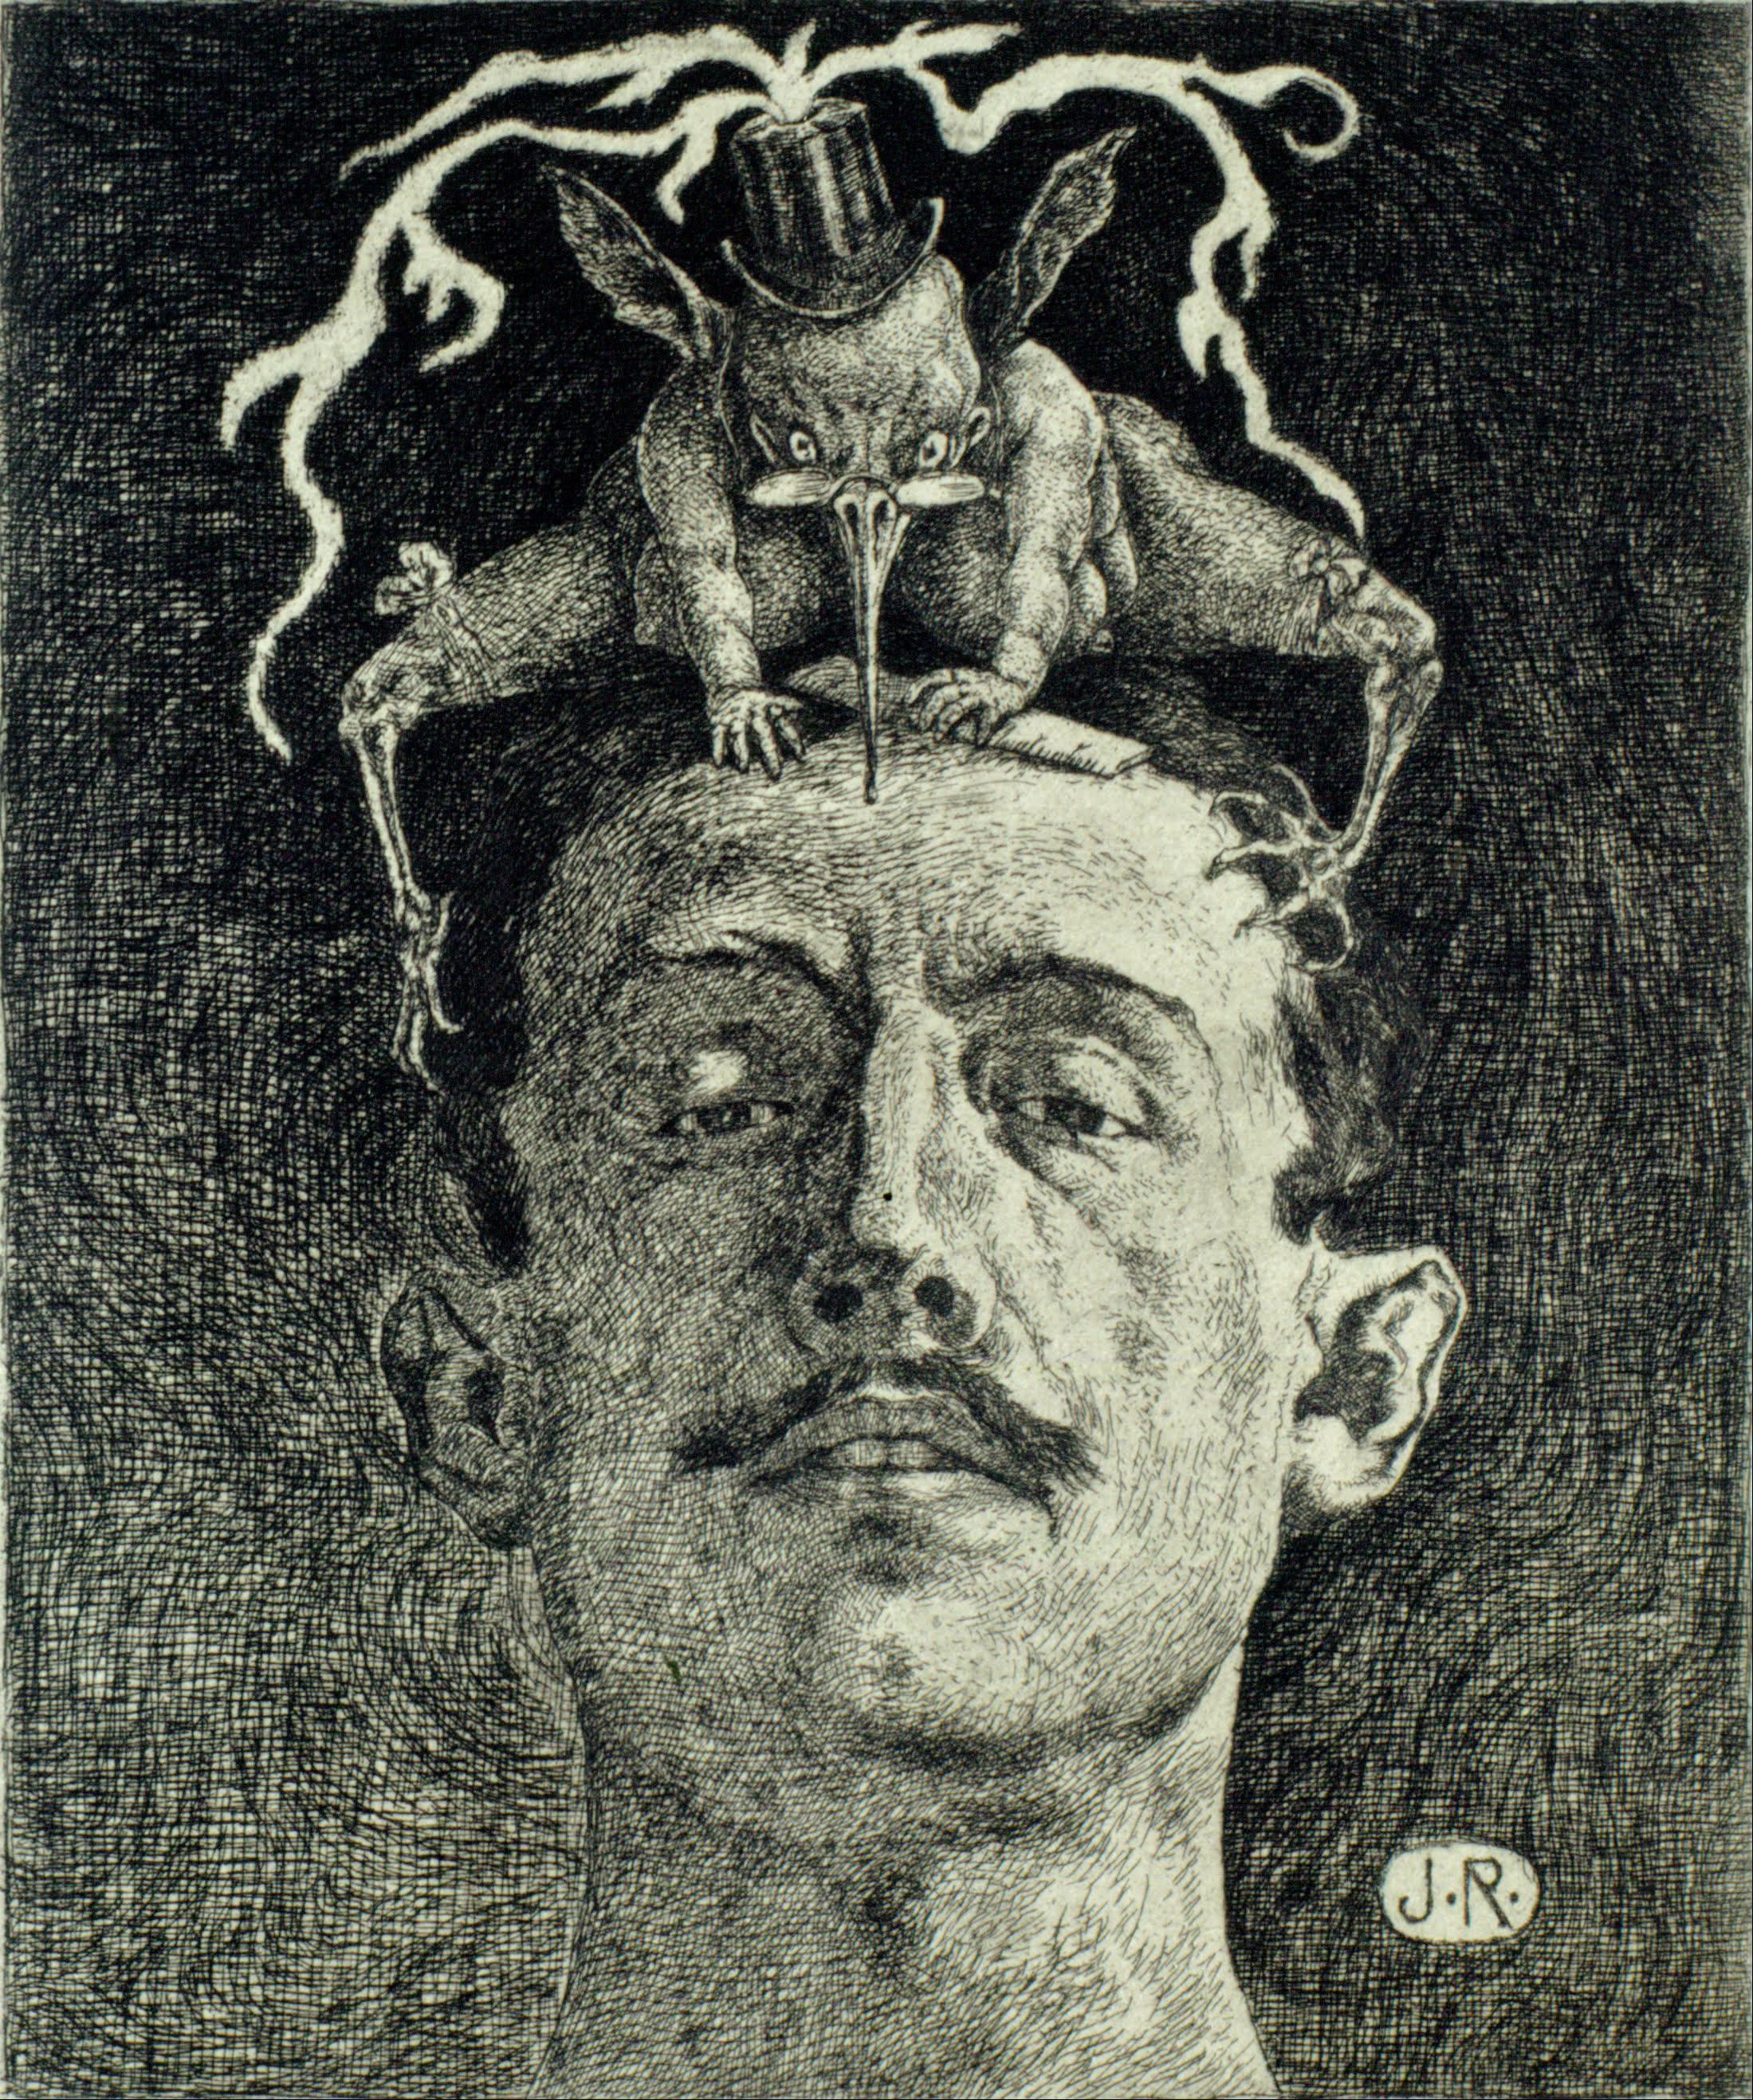
\includegraphics[width=0.3\textwidth]{innercritic}
  }
  \caption{Crítica by Julio Ruelas, ca. 1907}
\end{figure}

\vspace{1cm}

\noindent This thesis is a survey on the theory behind the machine learning
algorithm called \textit{generative adversarial networks} (GANs).

The purpose of the GAN algorithm is to train two neural networks through a
two-player, zero-sum game, hence the first chapter is on game theory.

The two neural networks model completely different functions. One is trained to
become a generative model and it is called the generator. The other is trained
to become an astute classifier between two classes (real data and generated
data) and it is called the discriminator. The value function $\V$ used by the
GAN algorithm can be understood through information theory, hence the second
section of this thesis is on information theory.

The original formulation of the GAN algorithm had some limitations in practice.
Some authors have made improvements to the original formulation by importing
theory from optimal transport. This is explored in the third section of this
thesis.

The GAN algorithm is best described as a framework for training two neural
networks, one to generate some type of data and another to judge how closely the
generated data resemble the real data. A generative model $g$ is a function that
takes data from one probability space $(\&Z, p_{\&Z})$, called the prior space,
and transforms it into something else entirely in some other probability space
$(\&X, p^*)$, called the target space.

\begin{definition}%
  \label{def:generator}
  Let $\Phi \subset \R^n$ be a space of parameter values. A
  \textnormal{\sffamily generator} $G$ is a function $G: \Phi \times \&Z \mapsto
  \target$, which maps $z$ drawn from $(\&Z, \pz)$ to $(\target, \pt)$. Let $\G$
  denote the generator parameterized by $\phi \in \Phi$.
\end{definition}

In the definition of the generator, we fixed a subset $\Phi \subset \R^n$ as the
space of parameter values which are optimized during training. The parameter
space for the discriminator is a different subset of $\R^n$, since the
discriminator is a very different type of neural network than the generator,
requiring a qualitatively different set of parameters. The space $\&X$ is the
output of the generator and is the input to the discriminator.

\begin{definition}%
  \label{def:discriminator}
  Let $\Theta \subset \R^n$ be a space of parameter values. A
  \textnormal{\sffamily discriminator} $D$, is a function
  $D: \Theta \times \target \mapsto [0, 1]$, which computes the
  probability that $x$ was drawn from $(\&X, \pt)$. Let
  $\D$ denote the discriminator parameterized by $\theta \in \Theta$.
\end{definition}

\begin{definition}
  The \textnormal{\sffamily generative adversarial networks} algorithm
  trains two neural networks, one called the generator $G$, which
  produces samples from the target space $(\&X, \pt)$ and the other,
  called the discriminator $D$, which computes the probability that an
  observed sample came from $(\&X, \pt)$.  We can put it all together
  in this diagram.
  \begin{center}
    \begin{tikzcd}
      \&Z \arrow{r}{G} & \tilde{\&X} \arrow{r}{} & (\&X, \tilde{\&X})
      \arrow{r}{D} & ([0, 1], [0, 1]) \arrow{r}{\V} & \R \\
      & \&X \arrow{ur}{} & {} & {} &
    \end{tikzcd}
  \end{center}
  $D$ maximizes and $G$ minimizes the value function,
  \begin{align}
    \label{eq:intro-V}
    \V = \mathbb{E}_{x \sim \pt}[{\log D_\theta(x})] +
    \mathbb{E}_{z \sim \pz}[\log{(1 - D_\theta(G_\phi(z)))}],
  \end{align}
  hence the GAN algorithm can be stated as
  \begin{align}
\min_\phi\max_\theta\mathbb{E}_{x \sim \pt}[{\log D_\theta(x})] +
    \mathbb{E}_{z \sim \pz}[\log{(1 - D_\theta(G_\phi(z)))}].
  \end{align}
\end{definition}

Many use cases for the GAN algorithm are in the generation of photo-realistic
images. Other use cases include medical imaging, where data sets often suffer
from class imbalances since it is easier to find data on healthy subjects. GANs
have been used to augment data sets by producing synthetic images of diseased
plant and animal tissues as in~\cite{ref:nazki-2018},~\cite{ref:valerio-2017},
and~\cite{ref:frid-2018}. Synthetic data may also help anonymize sources of data
for medical research, as explored in~\cite{ref:shin-2018}.

While most research focuses on the generative side of the algorithm, it is worth
keeping in mind that the GAN algorithm also produces a discriminator, which is a
classifier between two classes and has been used as a classifier
in~\cite{ref:cortes-2017} to classify different plant diseases, which was
inspired by~\cite{ref:odena-2016}.

To get a better sense of the significance of the GAN algorithm, we have provided
a quote from \cite{ref:goodfellow-original}.

\begin{quote}
  \itshape
  The generative model can be thought of as analogous to a team of
  counterfeiters, trying to produce fake currency and use it without detection,
  while the discriminative model is analogous to the police, trying to detect
  the counterfeit currency. Competition in this game drives both teams to
  improve their methods until the counterfeits are indistiguishable from the
  genuine articles.
\end{quote}

Unsurprisingly, the above is no longer an analogy and this competition between
counterfeiters and police is played out by the producers of fake images (and
videos) with nefarious intent (often used in fake news) and everyone else is
left scrambling to develop techniques to tell the real from the fake. See
\forloop{x}{1}{ \value{x}<11 }{ \cite{ref:df\arabic{x}}, } \cite{ref:df11} and
\cite{ref:df12} for more information on deep fake detection.

As stated above, the GAN algorithm comprises two artificial, feedforward neural
networks, a class of function made by composing many primitive functions.

\subsubsection*{Neural Networks}

\begin{definition}
  A \textnormal{\sffamily Feedforward Neural Network} is a directed graph. At
  each node is a composition of linear (or affine) functions with a nonlinear
  activation function. The input and output of the nodes are determined by the
  connectivity of the graph.
\end{definition}

\begin{figure}[H] \centering
  \begin{tikzpicture} \tiny
    %%% Nodes.
    \begin{scope}[]
      \matrix[nodes = {draw, nn}, column sep = 0.5cm] {
        \node (q1) {$q_1$}; &
        \node (q2) {$q_2$}; &
        \node (q3) {$q_3$}; &
        \node (q4) {$q_4$}; &
        \node (q5) {$q_5$}; \\
      };
    \end{scope}
    \begin{scope}[yshift = -1cm]
      \matrix[nodes = {draw, nn}, column sep = 0.5cm] {
        \node (r1) {$r_1$}; &
        \node (r2) {$r_2$}; &
        \node (r3) {$r_3$}; &
        \node (r4) {$r_4$}; \\
      };
    \end{scope}
    \begin{scope}[yshift = -2cm]
      \matrix[nodes = {draw, nn}, column sep = 0.5cm] {
        \node (s1) {$s_1$}; &
        \node (s2) {$s_2$}; &
        \node (s3) {$s_3$}; & \node (s4) {$s_4$}; \\
      };
    \end{scope}
    \begin{scope}[yshift = -3cm]
      \matrix[nodes = {draw, nn}, column sep = 0.5cm] {
        \node (x1) {$x_1$}; &
        \node (x2) {$x_2$}; &
        \node (x3) {$x_3$}; &
        \node (x4) {$x_4$}; \\
      };
    \end{scope}
    \begin{scope}[yshift = -4cm]
      \matrix[nodes = {draw, nn}, column sep = 0.5cm] {
        \node (y1) {$y_1$}; &
        \node (y2) {$y_2$}; &
        \node (y3){$y_3$}; \\
      };
    \end{scope}
    \begin{scope}[yshift = -5cm]
      \matrix[nodes = {draw, nn}, column sep = 0.5cm] {
        \node (z1) {$z_1$}; &
        \node (z2) {$z_2$}; &
        \node (z3) {$z_3$}; &
        \node (z4) {$z_4$}; &
        \node (z5) {$z_5$}; \\
      };
\end{scope}

%%% Edges.
\foreach \q in {1, 2, 3, 4, 5} {
  \foreach \r in {1, 2, 3, 4} {
    \path [line] (q\q) -- (r\r);
  }
}

\foreach \r in {1, 2, 3, 4} {
  \foreach \s in {1, 2, 3, 4} {
    \path [line] (r\r) -- (s\s);
  }
}

\foreach \s in {1, 2, 3, 4} {
  \foreach \x in {1, 2, 3, 4} {
    \path [line] (s\s) -- (x\x);
  }
}

\foreach \x in {1, 2, 3, 4} {
  \foreach \y in {1, 2, 3} {
    \path [line] (x\x) -- (y\y);
  }
}

\foreach \y in {1, 2, 3} {
  \foreach \z in {1, 2, 3, 4, 5} {
    \path [line] (y\y) -- (z\z);
  }
}
  \end{tikzpicture}
  \caption{A Deep Neural Network}
  \label{fig:deep_nn}
\end{figure}

If we let $f_\theta$ denote the neural network parameterized by $\theta \in
\Theta \subset \R^n$, we can think of training $f_\theta$ as searching through
the space of all possible parameters $\Theta$, in search of $\theta^*$ that
minimizes some differentiable measure of loss.

An information theoretic explanation for what deep learning is and how the
training works is given in \cite{ref:tishby-2015} and \cite{ref:tishby-2017}.
Tishby, Zaslavsky, and Shwartz-Ziv touch on some important topics in deep
learning from an information theory perspective. One such assertion of theirs is
the arbitrary nature of the structure of the graph, i.e.\ there are many
equivalent graphs that minimize the loss function, therefore we are not really
in search of some perfect $\theta^* \in \Theta$, as there are many equivalent
$\theta$.

There are many optimization algorithms for searching through $\Theta$, most of
which are variations of gradient descent. Gradients are taken with respect to
the loss function $\&L$ and the backpropagation algorithm assigns contribution
of error. \textit{Backpropagation} was introduced in \cite{ref:rumelhart-1986},
and is essentially an application of the chain rule of calculus to compute the
derivatives of the loss function with respect to each parameter in the graph. At
each node of the graph is a linear function, composed inside an activation
function, as in
\begin{align}
{1 \over 1 + \exp{\left(- \sum_{i = 1}^n x_i\theta_i - b \right)}}.
\end{align}
Like a neural network, a linear regression model is a function parameterized by
a set of learnable parameters $\theta$. The formula for linear regression is
\begin{align}
  \label{eq:lin-reg} \hat{y} = \sum_{i=1}^n x_i\theta_i - b.
\end{align}
The parameter vector $\theta$ of a linear regression model can be thought of as
an expression for how important each entry of $x$ is for a specific output $y$.
A linear regression model may also include a bias term $b$, which in the case of
a neural network can be interpreted as the activation threshold for the neuron.
In a sense, a neural network provides a way to compose many linear regression
models into a much larger model. \cite{ref:cheng-2018} even go so far as to say
that feed-forward neural networks are equivalent to polynomial regression.

\subsubsection*{Generative Adversarial Networks}

The generator of the GAN algorithm trains a generative model, which we define as
any mathematical or statistical model that mimics the process of creating the
observed data \cite{ref:bishop}. Starting with randomly initialized parameters,
which means we randomly choose a $\theta \in \Theta$, we optimize the model
until it maps random input into the desired output with frequencies similar
enough to the desired probability distribution.

The earliest reference to two-player games that result in the production of a
generative model can be found in \cite{ref:doyle}, a short article containing
the following game. \textit{``We are told the constraints, we pick a
  distribution, God gets to pick the `real' distribution, satisfying the
  constraints of course. Some disinterested party picks an outcome according to
  the `real' distribution that God has just picked, and we have to pay according
  to how surprised we are to see that outcome.''} This is not quite the GAN
algorithm, but it has a similar moral, that is we seek a probability
distribution and we learn what qualities define it through feedback. If we
iterate the above procedure and formalize a way of learning from our surprise,
we arrive at something resembling the GAN algorithm.

As for the history of adversarial games (where the players are trying to
undermine each other), J\"{u}rgen Schmidhuber wrote more than one paper, the
first of which appeared in 1992, on what he called \textit{predictability
  minimization}, which is very similar to the GAN algorithm (see
\cite{ref:schmidhuber-1992} and \cite{ref:schmidhuber-2018}). The idea behind
predictability minimization was for one player to try to predict outcomes in
some event space and the adversary tries to minimize the ability of that player
to make those predictions.

A blog post from 2010 \cite{ref:niemitalo-2010} essentially describes the GAN
algorithm. In 2012, a paper on adversarial support vector machines was written
by \cite{ref:zhou-2012}. Finally, in 2014 an algorithm for training models to
simulate the behavior of animals based on two populations, replicas and
classifiers, was written by \cite{ref:li-2014}.

In 2014, while a student of Yoshua Bengio at the Universit\'{e} de Montr\'{e}al,
Ian Goodfellow and colleagues published \textit{Generative Adversarial Nets}.
This paper has since inspired many publications and has triggered a surge in the
interest in generative models.

Now with this thesis we present a survey of the mathematical theory behind
Generative Adversarial Networks. The relevant theories discussed are game
theory, information theory and optimal transport theory.

%%% Local Variables:
%%% mode: latex
%%% TeX-master: "../thesis"
%%% End:
